\section{How information crosses the boundary}
\label{sec:seam}

Three problems are often treated as one.
\begin{itemize}
  \item \emph{Local inference:} what do a module's own data say about its own
  parameters?
  \item \emph{Uncertainty propagation:} given the uncertain output of one module,
  how uncertain is the next module?
  \item \emph{Cross-module inference:} do the data of one module inform the
  parameters of another, when the two share no parameter?
\end{itemize}
The third problem is the hard one. This section maps what we know of it. Our claims
in \cref{sec:results} rest on calibration on M0, and not on a measured transfer of
information across the boundary by the exact sampler.

\subsection{Three graphs}

A coupled model has three graphs, and they need not agree
(\cref{fig:graphs}). The \emph{coupling graph} says which module drives which
state. The \emph{likelihood graph} says which likelihood factors depend on which
parameters once the stochastic paths are integrated out. The \emph{information
graph} says which data streams move which parameters. In the reduced \syn{} model the
coupling graph is two-way, but the information graph is sparse and points mostly in
one direction.

\begin{figure}[!ht]
\centering
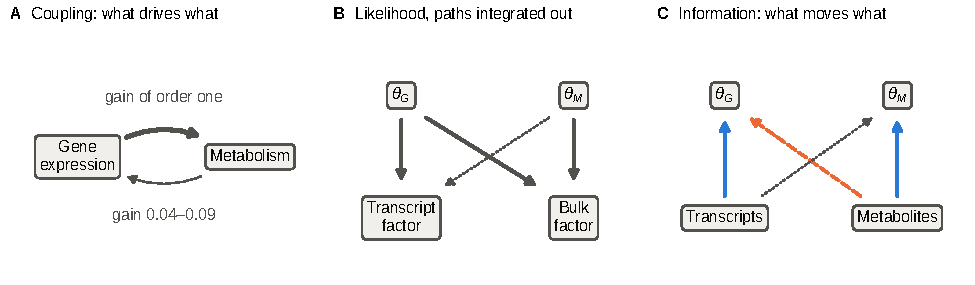
\includegraphics[width=\textwidth]{fig_graphs.pdf}
\caption{\textbf{Three graphs of one model.} A: the coupling is two-way, with a strong drive
from gene expression to the pools and a weak one back. Line width shows gain. B: once the
paths are integrated out, the gene-expression parameters $\theta_G$ enter both factors,
and the metabolic parameters $\theta_M$ reach the transcript factor only weakly (dotted). C:
what the data move. Solid: each stream informs its own module, on both routes. Dashed: metabolites
to gene expression, shown by the linearised bound and the mixed route, with no exact result.
Dotted: transcripts to metabolism, a null read-off on M0.}
\label{fig:graphs}
\end{figure}

Write $u$ for the trajectory at the interface: enzyme counts and drains in one
direction, pools in the other. For a pair of modules $A \to B$ with data $D_A$ and
$D_B$, the forward message is $p(u \mid D_A)$. The backward message is a likelihood
over the interface. For a one-way coupling, with $D_A$ and $D_B$ independent given $u$, \begin{equation}
  \lambda_B(u) = \int p(D_B \mid \theta_B, u)\, p(\theta_B)\, \mathrm{d}\theta_B .
\end{equation}
The joint posterior over $u$ is proportional to $p(u \mid D_A)\,\lambda_B(u)$. With feedback, as here, the messages alternate rather than close in one pass. A
\emph{statistical cut} drops $\lambda_B$ \cite{plummer2015cuts}. It changes the
target of inference, and data from $B$ can no longer inform $A$. A \emph{dynamical
reduction} instead removes a weak edge from the simulator and keeps full Bayesian
inference. For the question we ask, only the second kind keeps the information we
want: metabolite data that inform a gene-expression parameter.

\subsection{Information follows gain}

The strength of each coupling direction predicts where information flows
(\cref{tab:gain}). From gene expression to the pools the gain is of order one. The
pools turn over in seconds to minutes, and the drains from gene expression are a
large part of that turnover. From the pools back to the rate constants the gain is
small: an elasticity of \pn{gain.txlo}--\pn{gain.txhi} for transcription and
\pn{gain.tl} for translation. The gain is small because the published rate laws are
saturated. The elasticity here is $\partial \ln k / \partial \ln c$, of a rate constant $k$ in a pool $c$. The published law's dissociation constant $K_d$ for RNA polymerase and its nucleotides is \pn{gain.kd}\,mM, while ATP is near \pn{gain.atp}\,mM.

\begin{table}[!ht]
\caption{\textbf{Gain and information in each direction across the boundary.} Information is the ratio of posterior to prior standard deviation at 200 cells. The ptsG value is a linearised bound at 10\% assay noise, and its bracket is the ratio that noise alone gives. The ENO value is a Gaussian approximation from the path's Fisher information, linearised at one truth, from 40 cells scaled to 200, with no assay noise.}
\label{tab:gain}
\centering
\small
\begin{tabular}{@{}p{0.3\columnwidth}p{0.25\columnwidth}p{0.33\columnwidth}@{}}
\toprule
Direction & Gain & Information \\
\midrule
Gene expression $\to$ pools & order one & ptsG from metabolites only: \pn{info.ptsg} (bracket \pn{info.ptsgbracket}) \\
Pools $\to$ rate constants & \pn{gain.txlo}--\pn{gain.txhi} (transcription), \pn{gain.tl} (translation) & ENO from transcripts only: \pn{info.enotx} \\
\bottomrule
\end{tabular}
\end{table}

So the linearised bound says that metabolite data can inform the ptsG promoter, a
gene-expression parameter that they never measure. On M0 the mixed route shows this
shrinkage, to \pn{mix.ptsgbulk} of the prior standard deviation. That is less shrinkage than the bound of \pn{info.mzeroptsg} projects, and that calculation's own split-half noise ratio is \pn{info.mzerobracket}. The exact fit under metabolites only did not mix for
this parameter, so on the exact sampler this direction is unmeasured, and we do not claim
it there. Transcript data carry almost no information about the enolase constant, a
metabolic parameter. We report that result as a null, not as a failure. On M0 at \pn{mzero.cells} cells, the exact sampler's divergence under
transcripts only is \pn{tsplit.eno}\,nat for enolase and \pn{tsplit.fba}\,nat for
aldolase, each below its noise floor. That read-off is M0's. We did not run the
planned test at 1,000 cells, so we do not extend it to the full reduced model.

\subsection{Why no parameter is shared}

The standard modular methods pass messages through shared parameters: cuts and
semi-modular inference \cite{plummer2015cuts,carmona2020semimodular}, and Markov
melding \cite{goudie2019joining}. In the reduced model no parameter is shared, so
these methods have nothing to pass while we condition on the stochastic path. The
exact sampler does what is left: it conditions on the path, and it updates the path
with all the data. In this sense the exact sampler is modular inference with nothing
dropped. When the paths are integrated out, a gene-expression parameter appears in
both the transcript factor and the metabolite factor. The mixed route uses this
structure.
